\chapter{Software Testing}

\section{Warum ist Testen so wichtig}

Werden Tests nicht schon von Beginn weg eingeplant, werden sie nie mehr aufgeholt. Der Zeitverzug führt dazu, dass selbst die bestehenden Tests nur rudimentär durchgeführt werden. Es fehlt meist die zugeordnete Verantwortlichkeit (Rolle) welche sicherstellt, dass Tests auf Vollständigkeit, Sinnhaftigkeit und Realitätsbezug erarbeitet und durchgeführt werden. Damit man erfolgreich Testen kann braucht es drei Dinge:
\begin{description}
	\item[Test-Tool] Tools gibt es wie Sand am Meer. Aus der Sicht des Managements sind Tools ideal, weil sie ein Preisschild haben und es sich um eine einmalige Investition handelt. Zudem wird das Personalbudget nicht belastet und die Tool-Hersteller wollen verkaufen und argumentieren deshalb gut. Das hat zur Folge das gerne und viel in Tools investiert wird. 
	\item[Prozess] Prozesse sind in einem Unternehmen meist schon vorhanden. Prozesswissen ist vorhanden und es muss immer ein Hype (ITIL, SCRUM usw.) verwendet werden. Investitionen erübrigen sich, da Prozesse nur \textit{gemalt} werden müssen. Für eine firmenweite Prozessdoku reicht meist das Geld nicht. Deshalb wird in diesem Bereich weder aktiv investiert noch aktiv gespart.
	\item[Testmanager] Die Schlüsselrolle des Testmanagers wird oft verkannt, weil theoretisch jeder testen kann. Dadurch verkommt Testen oft zum \textit{Anhängsel}. Personal kostet und deshalb wird nur in Entwickler investiert, welche die gewünschten Anforderungen in Code umsetzen. Testen können am Schluss die künftigen Anwender. Personalkosten sind nicht gern gesehen im Budget, denn was macht man mit dem ganzen Personal nach Projekt-Ende? Die Personalbeschaffung übersteigt auch oft die Budgetkompetenz eines Projektleiters. Hier wird selten investiert, aber auch sehr schnell gespart.
\end{description}
Diese ungerechte Verteilung kommt zustande, weil nur die aktuellen Investitionskosten im Vordergrund stehen. Allfällige Kosten welche durch Fehler entstehen, fallen unter ein anderes Budget. Deshalb sind diese Kosten meist nicht auf dem Radar der Entscheidungsträger. Zudem kann der Nutzen von Testen nicht quantifiziert oder belegt werden. Auch die Tester argumentieren meist zu technisch und zu wenig ökonomisch.

Wenn beim Testen gespart wird geht oft einiges schief. Testtools sind beispielsweise nicht optimal konfiguriert und nicht an das Unternehmen (Prozess, Kultur) angepasst. Dadurch dass die Testtools nicht gepflegt und gewartet werden, entstehen viele Leichen, also Tools die zwar vorhanden sind aber nicht verwendet werden. Die Prozesse passen meist nicht auf aktuelle Abläufe weil sie zu starr modelliert sind. Da sie nicht verbessert werden, behindern sie zügiges Arbeiten. \textbf{Es fehlt das Aktive, die Verantwortlichkeit und die Führung}.

Das Testen beginnt mit der Abnahme (Freigabe) der Anforderungen. Wichtig ist dabei dass der Endzustand klar, vollständig und widerspruchsfrei beschrieben ist. Die Abnahme der Anforderungen sollte deshalb von einem Team übernommen werden, welches Kompetenzen aus Entwicklung, Architektur, Testengineering, Fachverständnis und Support mitbringt. Das Testengineering stellt sicher, dass Anforderungen vollständig, widerspruchsfrei und messbar sind. 

Ein Softwaretest prüft und bewertet Software auf Erfüllung der für ihren Einsatz definierten Anforderungen und misst ihre Qualität. Dazu passt auch folgender \textit{Spruch}:
\begin{quote}
	Testen unterscheidet sich von Experimentieren dadurch, dass es beim Testen eine Erwartung gibt die belegt werden soll, während das Ergebnis beim Experimentieren offen ist oder nur vermutet werden kann.
\end{quote}

Dem V-Modell aus Abbildung \ref{fig:v-modell} lässt sich entnehmen, dass auf jeder Ebene der Entwicklung das Testen nötig ist.
\begin{figure}[h!]
\centering
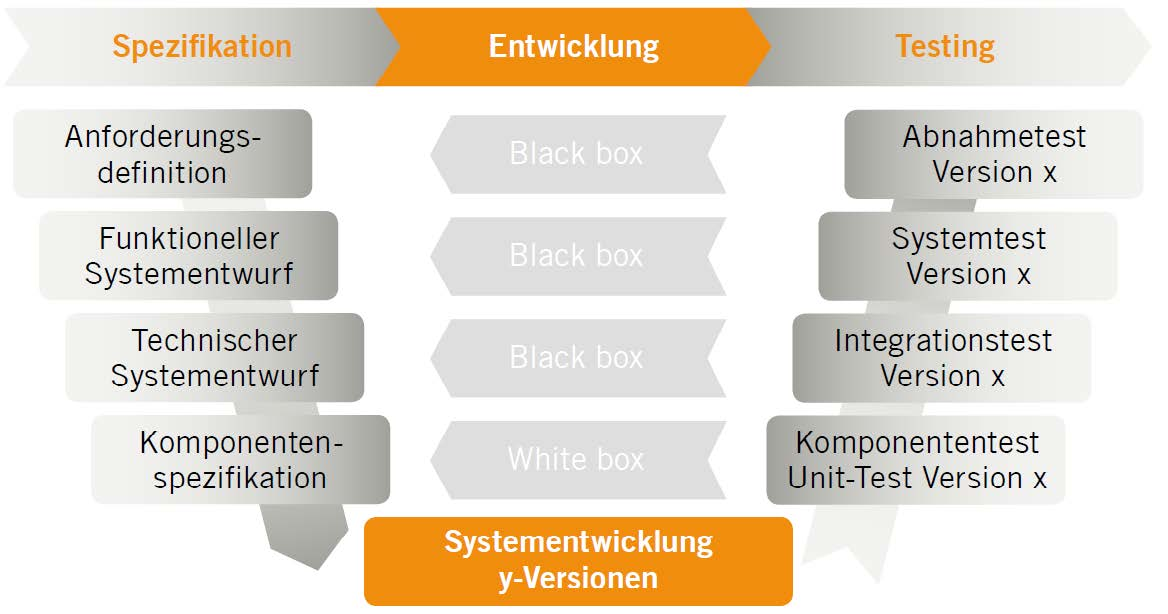
\includegraphics[width=0.7\linewidth]{fig/v-modell}
\caption{V-Modell}
\label{fig:v-modell}
\end{figure}
Zudem gibt es eine ISO-Norm (Abbildung \ref{fig:iso-25000}), die beschreibt wie Qualität aussieht.
\begin{figure}[h!]
\centering
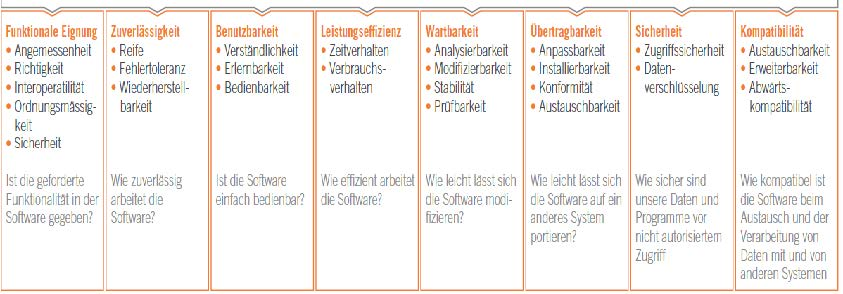
\includegraphics[width=0.5\linewidth]{fig/iso-25000}
\caption{Qualitätsnorm}
\label{fig:iso-25000}
\end{figure}

Eine weitere interessante Beobachtung ist, dass bei schlechten Tests und einem schlechten Produkt wenig Fehler gefunden werden, weil die Tests nicht alle Fehler einfangen. Wenn man dann die Qualität der Tests erhöht, findet man sehr viele Fehler. Erst wenn auch die Qualität der Software erhöht wird findet man wieder wenig Fehler.

Auch in agilen Projekten hat Testen durchaus seinen Platz, denn Sinn und Zweck des Testens ist unabhängig von der verwendeten Projektmethode. Jedoch muss die Organisation des Testens an die Projektmethode angepasst werden. In agilen Projekten kann pro User Story ein Test-Case erstellt werden. In den darauffolgenden Iterationen wird dieser Test-Case immer weiter angepasst bis er evtl. sogar automatisiert werden kann. Bei einem Wasserfall-Projekt ist das Test- und Entwicklungsteam getrennt. Die beiden Teams arbeiten in unterschiedlichen Welten, was oft zu mangelhafter Synchronisation zwischen den Teams führt. Mit dem Testen wird auch oft zu spät begonnen, was meistens zu kostspieligen Fehlern führt. 

Das Testen hat sich im Laufe der Zeit verändert. Das Testmanagement hat sich von der reinen Prüfdisziplin zum Steuerungsinstrument für nachhaltige Systemqualität entwickelt. Probleme können effektiv verhindert werden, weil Fehler früh erkannt und behoben werden können. Das Management hat mit dem Testmanager eine kompetente Ansprechperson, um mit seiner Hilfe fundierte Entscheidungen zu treffen. Durch das Testen wird Transparenz geschaffen was den Entscheidungsprozess beschleunigt und dadurch Wettbewerbsvorteile verschafft werden.

\subsection{Der Nutzen von Testen}

\begin{itemize}
	\item Das Testbudget kann eingeplant werden, Kosten für Nachbesserungen nicht.
	\item Fehler kosten Geld, Testen stellt sicher, dass Fehler früher systematisch erkennt werden.
	\item Ein konsequent gelebter Testprozess hat auch positiven Einfluss auf die Beschreibung der Anforderungen - es kann schlussendlich schneller entwickelt werden.
	\item Mittels eines Testprozess ist man gezwungen, dass Fehler, Änderungen und Neuanforderungen genau umschrieben werden.
	\item Testmanagement ist Führungsarbeit und gerade in agilen Prozessen dank nachweisbaren Fakten oft das einzig stete und somit verlässliche.
\end{itemize}

\begin{figure}[h!]
	\centering
	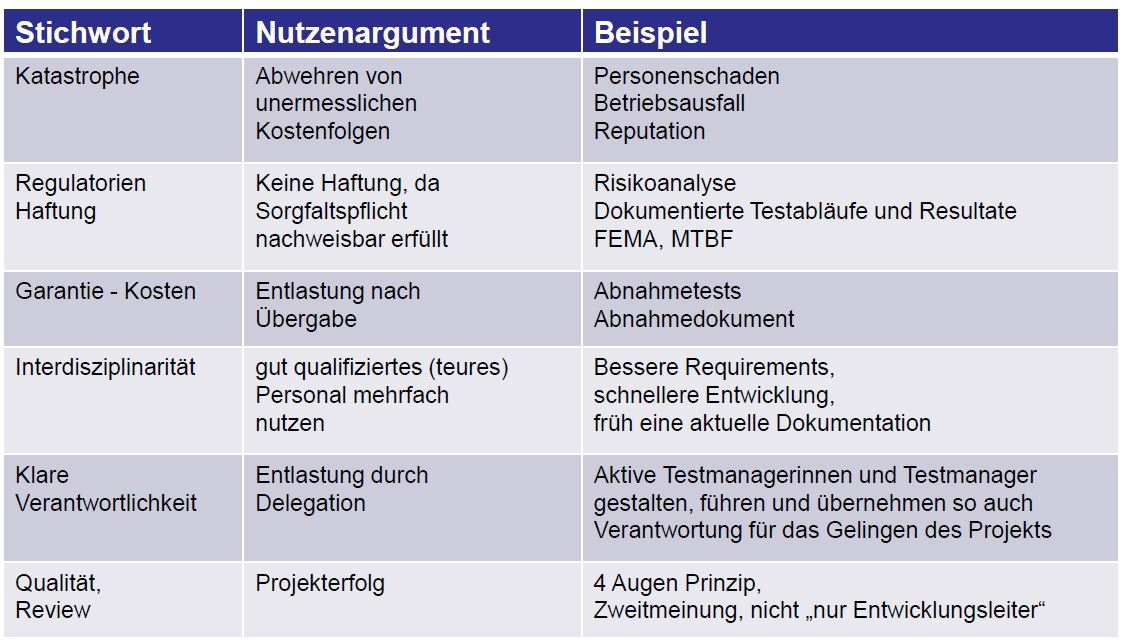
\includegraphics[width=0.7\linewidth]{fig/testen-nutzen-1}
	\caption{Testen Nutzen 1}
	\label{fig:testen-nutzen-1}
\end{figure}

\begin{figure}[h!]
	\centering
	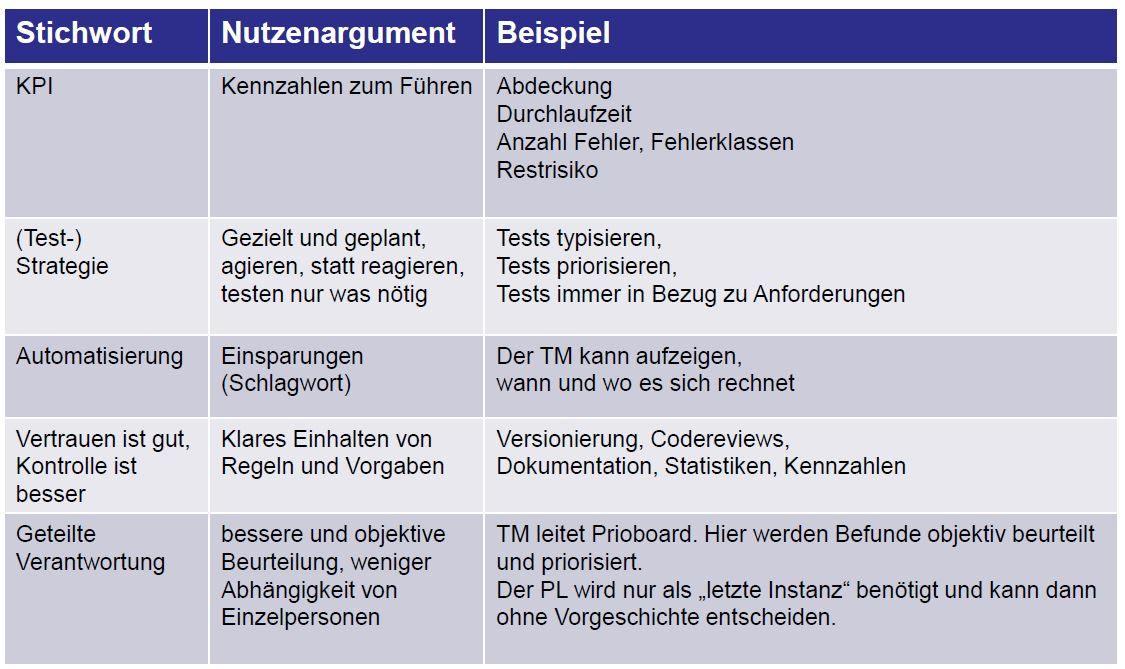
\includegraphics[width=0.7\linewidth]{fig/testen-nutzen-2}
	\caption{Testen Nutzen 2}
	\label{fig:testen-nutzen-2}
\end{figure}


\section{Test-Prozess}

Innerhalb des Test-Prozess arbeiten mehrere Personen mit unterschiedliche Rollen:

\begin{description}
	\item[Testmanager (Führung)] Ansprechpartner für PL und Managemenet in kritischen Phasen. Plant Ressourcen, sucht verschiedene Lösungen und bewertet sie. Kann Leute führen. Entwickelt Teststrategien.
	\item[Testarchitekt, Testengineer (Ingenieur)] Plant und entwickelt die Testinfrastruktur. Entwickelt und verbessert Testmethoden und Testwerkzeuge. Entwickelt Teststrategien.
	\item[Testanalyst (Ingenieur)] Leitet aus Anforderungen Testszenarien ab. Entwickelt komplexe Testabläufe. Bestimmt Testdaten.
	\item[Testdatenverantwortlicher (Informatiker)] Pflegt, verwaltet, bewirtschaften und erweitert die Testdaten mittels Tools. Schnittstelle zwischen Testanalysten, Fach und IT. 
	\item[Tester (Fachperson)] Führt zuverlässig und exakt Tests aus. Dokumentiert präzis und wertfrei/neutral die Ergebnisse sowie die Abweichungen. Kann reproduzieren.
\end{description}

Wie die Abbildung \ref{fig:test-prozess} zeigt, ist der Test-Prozess (nach Noser) in vier Schritte eingeteilt.

\begin{figure}[h!]
\centering
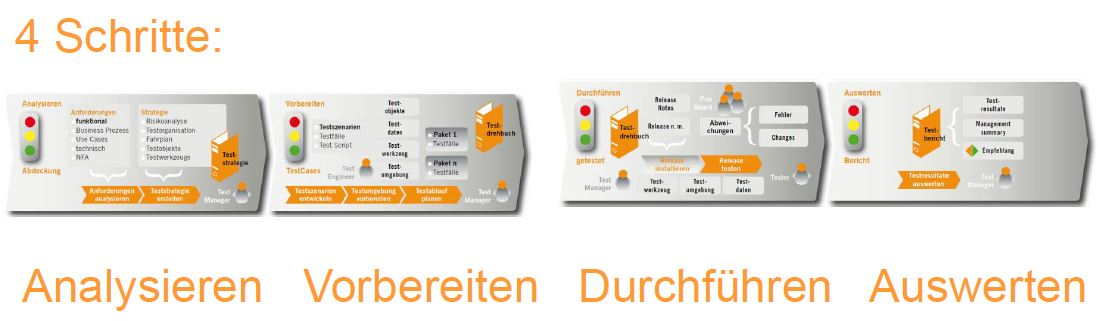
\includegraphics[width=0.7\linewidth]{fig/test-prozess}
\caption{Test-Prozess}
\label{fig:test-prozess}
\end{figure}

\subsection{Schritt 1: Analysieren}

\textit{Wie können die Entwickler entwickeln, wenn die Tester nicht wissen, was zu testen ist?}


\begin{figure}[h!]
\centering
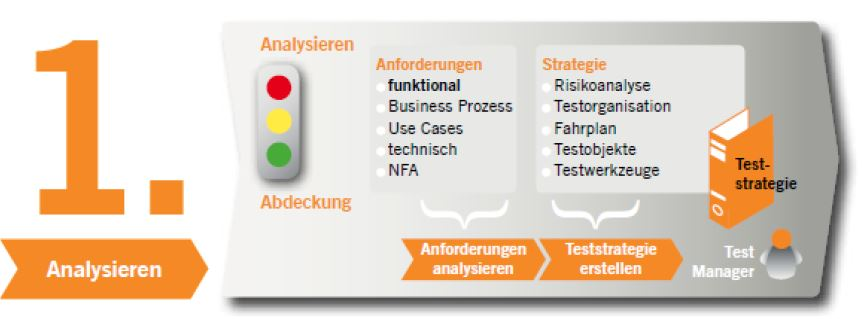
\includegraphics[width=0.7\linewidth]{fig/test-prozess-schritt-1}
\caption{Test-Prozess Schritt 1}
\label{fig:test-prozess-schritt-1}
\end{figure}

\textbf{Testen braucht eine Strategie}. Die Teststrategie bestimmt ob, was und wie tief getestet werden soll. Wo liegt der Fokus? Preis, Durchlaufzeit, Security, Usability, Performance, etc.? Vorgängig soll man sich darüber Gedanken machen und diese verbindlich festhalten. In der Teststrategie wird das Test-Vorgehen, verantwortliche Personen sowie den Prozess und die Hilfsmittel definiert. 

Warum ein Risiko basiertes Testen: Oft bleibt in kritischen Phasen nicht genug Zeit um \emph{alles} zu testen. Daher pro Iteration entscheiden, was in welchem Umfang getestet wird - kategorisieren und priorisieren. Nachfolgend werden drei Kriterien mit einem Wert von 1-3 bewertet. Das Produkt daraus gibt den Risiko Prioritäts Index (RPI):

\begin{itemize}
	\item Business Relevanz: Auswirkung bei Fehler, wie schlimm ist ein Fehler (3 = am schlimmsten)
	\item Auffindbarkeit: Wie schnell wird ein Fehler entdeckt? (1 = leicht erkennbar)
	\item Komplexität: Wie komplex ist die Anforderung und die Lösung dazu? (3 = sehr komplex)
\end{itemize}

\begin{figure}[h!]
\centering
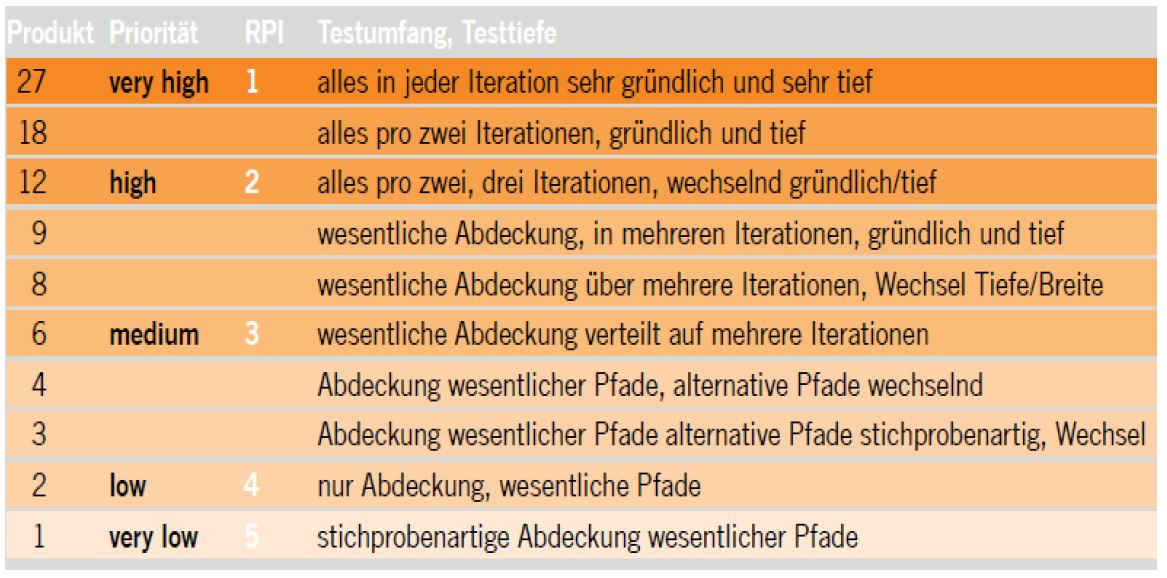
\includegraphics[width=0.8\linewidth]{fig/rpi-skala}
\caption{RPI-Skala}
\label{fig:rpi-skala}
\end{figure}

Der RPI definiert die Testtiefe, den Testumfang und die Anzahl der Wiederholungen. Somit ist der RPI das wichtigste Steuerungs- und Führungsinstrument.

Nebst dem Risiko basierten Testen gibt es noch andere Teststrategien:

\begin{itemize}
	\item ISO 29119: Was umfasst Qualität. Umfassende und ganzheitliche Betrachtung. Nach Vorlagen - Rad nicht neu erfinden.
	\item V-Modell: Tests auf jeder Stufe. Fehler so früh wie möglich entdecken.
	\item RPI: Risikiobasiertes Testen. So wenig wie möglich, aber das wo nötig.
	\item Kosten-Nutzen: Risikoabwägung. Welches Risiko wollen wir tragen, was darf es kosten?
\end{itemize}

Nebst dem Vorgehen spielen auch die \textbf{Tools} eine wichtige Rolle. Welche Tools werden für die Verwaltung von Anforderungen, Tests, Testabläufe und Testplanung verwendet. Mit was macht man Bug-Tracking, manuelles Testen, automatisiertes Testen, Lasttest, Datenmanipulation, Datengenerierung? Für alle Tools sollte man sicher immer Gedanken machen. Was ist das Ziel, wer kann das Tool bedienen, wie sieht die Lebensdauer aus, Kosten, wartbar, etc.

\newpage

\subsection{Schritt 2: Vorbereiten}

\textit{Tester und Q-Menschen sind nie bereit, sie können die Testvorbereitung sowie die Testinfrastruktur problemlos vergolden.}

\begin{figure}[h!]
\centering
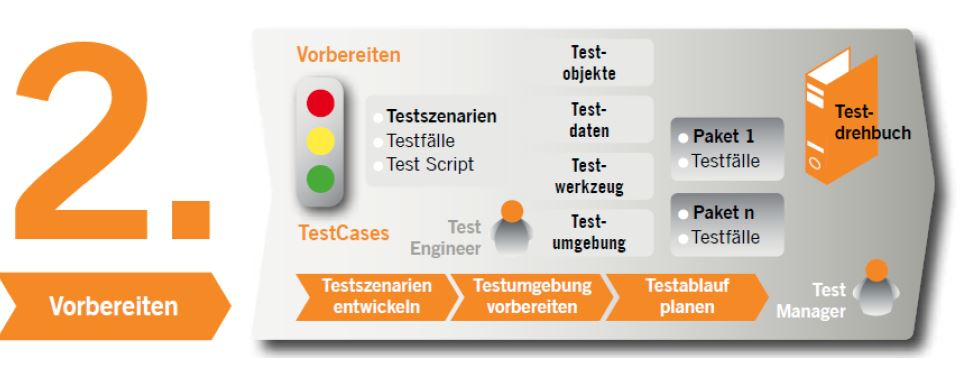
\includegraphics[width=0.7\linewidth]{fig/test-prozess-schritt-2}
\caption{Test-Prozess Schritt 2}
\label{fig:test-prozess-schritt-2}
\end{figure}

Die Vorbereitungsphase legt die Basis für den Erfolg:

\begin{itemize}
	\item Test-Infrastruktur
	\item Test-Team (keine Diletanten!)
	\item Test-Daten
	\item Test-Automaten, Test-Automatisierung
	\item Eskalationswege
	\item NFA-Test
	\item Test-Stufen
	\item Test-Szenarien, Test Cases, Test-Fälle
\end{itemize}

\begin{figure}[h!]
\centering
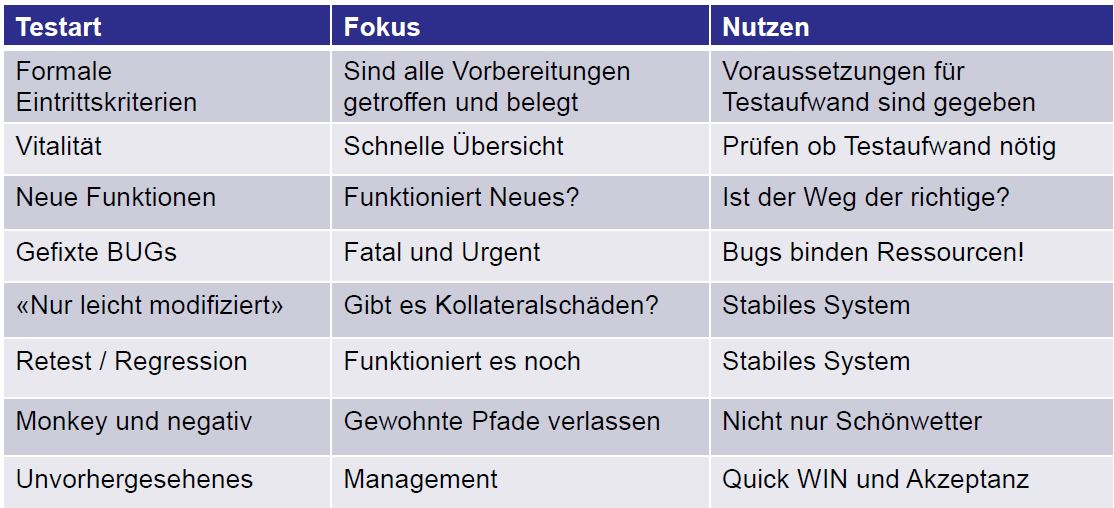
\includegraphics[width=0.7\linewidth]{fig/testarten-zur-planung}
\caption{Testarten zur Planung}
\label{fig:testarten-zur-planung}
\end{figure}

Mittels Blackbox-Test wird das Ein- und Ausgabeverhalten überprüft. Dabei kann die Anzahl der Testfälle explodieren. Mittels Whitebox-Test werden die interne Logik des Systems oder Objekts angeschaut. 

Die Codeabdeckung ist eine Metrik, welche die die durch Tests erreichte Codeabdeckung beschreibt. Damit können die benötigten Testfälle ermittelt werden. Es gibt unterschiedliche Abdeckungen:
\begin{description}
	\item[Anweisungsüberdeckung] Jede Anweisung wird mind. 1 mal aufgerufen.
	\item[Zweig-, Entscheidungsabdeckung] Jeder Eintritt- und Austrittspunkt wird mind. einmal durchlaufen.
	\item[Pfadabeckung] Pfade im Code.
\end{description}

Wir können nicht alles testen, da es unzählige Pfade gibt. Wir brauchen eine Strategie, welche risikobasiert ist um die Frage zu beantworten, wie viel und wie tief getestet werden soll.

\subsection{Schritt 3: Durchführen}

\textit{Die Praxis zeigt immer wieder, dass von Hand gepflegte Systeme in kritischen Momenten nicht mehr gepflegt werden, denn Testen geht immer vor. Doch genau dann sind die Kennzahlen als Entscheidungsbasis besonders wichtig.}

\begin{figure}[h!]
\centering
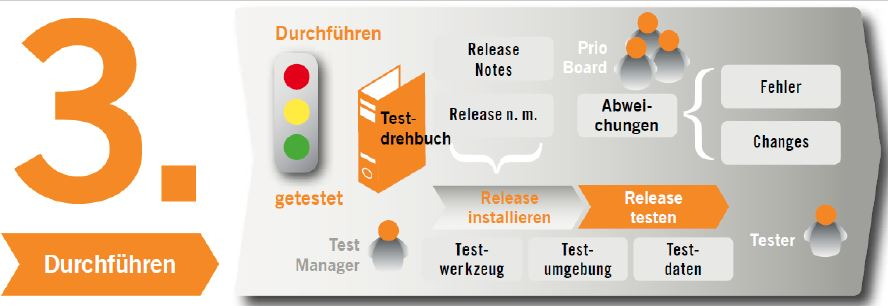
\includegraphics[width=0.7\linewidth]{fig/test-prozess-schritt-3}
\caption{Test-Prozess Schritt 3}
\label{fig:test-prozess-schritt-3}
\end{figure}

Auf Abbildung \ref{fig:wichtigkeit-des-testen} sieht man, dass sowohl der linke untere Quadrant und der rechte obere Quadrant dasselbe Ergebnis liefern. Das ist trügerisch!

\begin{figure}[h!]
\centering
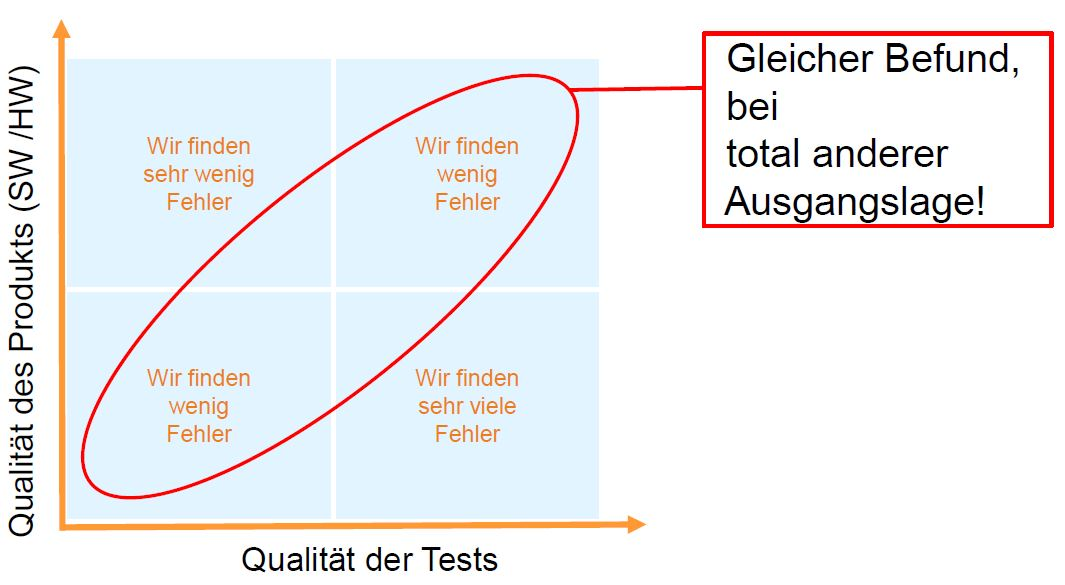
\includegraphics[width=0.7\linewidth]{fig/wichtigkeit-des-testen}
\caption{Wichtigkeit des Testen}
\label{fig:wichtigkeit-des-testen}
\end{figure}

Agile Methoden setzen auf das Testen als Mittel zur Fortschrittsmessung. Schlussendlich wird das Testen innerhalb der Definition of Done formuliert. Ein erfolgreicher Test belegt faktenbasiert, dokumentiert, reproduzierbar und emotionslos, den tatsächlichen Stand/Fortschritt des Projekts. Wobei man im agilen Umfeld mit folgenden Problemen kämpft: Anforderungen nicht sauber definiert, nebst dem Schreiben des Codes geht das Test schreiben unter. Es fehlt die Rolle des Testmanager, kein Reporting.

Abbildung \ref{fig:der-bug} zeigt dass ein Bug nicht unbedingt ein Bug sein muss. Ein wirklicher Bug zahlt die Entwicklungsfirma. Bei einem Change kann man sich streiten wer zahlt. Bei einer neuen Anforderung zahlt der Kunde.

\begin{figure}[h!]
\centering
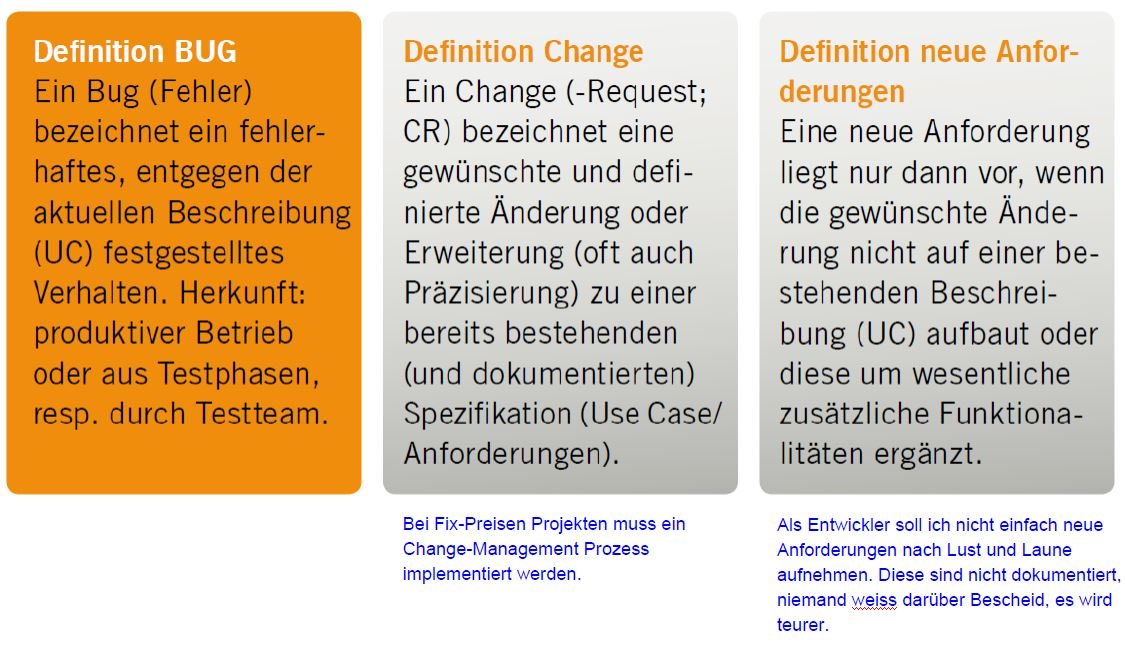
\includegraphics[width=0.7\linewidth]{fig/der-bug}
\caption{Der BUG (MEP!)}
\label{fig:der-bug}
\end{figure}

Ist jeder Fehler ein Fehler? Es macht Sinn die Fehler mit einer Severity (Schweregrad) kategorisieren:
\begin{description}
	\item[1 LOW:] leichter Fehler, nur einzelne Testschritte betroffen.
	\item[2 MEDIUM:] Betriebsstörender Fehler, Systemfunktion nicht beeinträchtig.
	\item[3 HIGH:] Schwerer Fehler, Auswirkung auf Funktion.
	\item[4 URGENT:] Fataler Fehler, Auswirkung auf ganzes System, Testabbruch.
\end{description}

Zudem stellt sich immer die Frage ob die Fehler reproduzierbar sind. Man spricht von \textbf{Beobachtungsgüte}:
\begin{itemize}
	\item A: Eindeutig festgestellter, belegbarer und reproduzierbarer Fehler.
	\item B: Nicht ohne weiteres reproduzierbar, aber wiederholt aufgetreten.
	\item C: Nicht reproduzierbar.	
\end{itemize}

\subsection{Schritt 4: Auswerten}

\begin{figure}[h!]
	\centering
	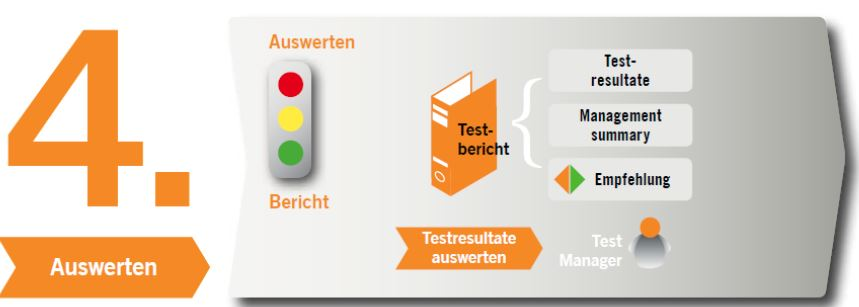
\includegraphics[width=0.7\linewidth]{fig/test-prozess-schritt-4}
	\caption{Test-Prozess Schritt 4}
	\label{fig:test-prozess-schritt-4}
\end{figure}

Der letzte Schritt ist eine Auswertungsphase, in der die Testresultate zu \textit{management-tauglichen} Reports zusammengefasst und grafisch dargestellt. Der Testreport soll dem Management ermöglichen, basierend auf dem zu erwartenden Restrisiko eine Entscheidung betreffend Go/NoGo zu treffen. Nachfolgend sind ein paar Kriterien aufgelistet, die beachtet werden sollten bezüglich den Go/NoGo-Entscheides:
\begin{itemize}
	\item Wer fällt die Entscheide
	\item Gibt es eine Überraschung
	\item Wie werden die Entscheide gefällt
	\item Existieren Fakten
	\item Ist ein Entscheid begründbar
	\item Ist ein Entscheid nachvollziehbar
	\item Sind mögliche Risiken identifiziert und bekannt
	\item Gibt es Entscheidungskriterien
	\item Wird aus dem Bauch entschieden
\end{itemize}
Ein Beispiel für einen Report findet man in Abbildung \ref{fig:go-nogo-report}. Dabei wurden Komponenten mit einem hohen Risiko (RPI 1) komplett mit Tests abgedeckt und es befinden sich keine bekannten Fehler mehr in der Komponente. Komponenten mit einem tieferen Risiko werden nicht komplett mit Tests abgedeckt und teilweise sind sogar noch kleine Fehler vorhanden, welche aber das Produkt nicht beeinflussen. Durch diese Darstellung kann das Management eine fundierte Entscheidung treffen.
\begin{figure}[h!]
\centering
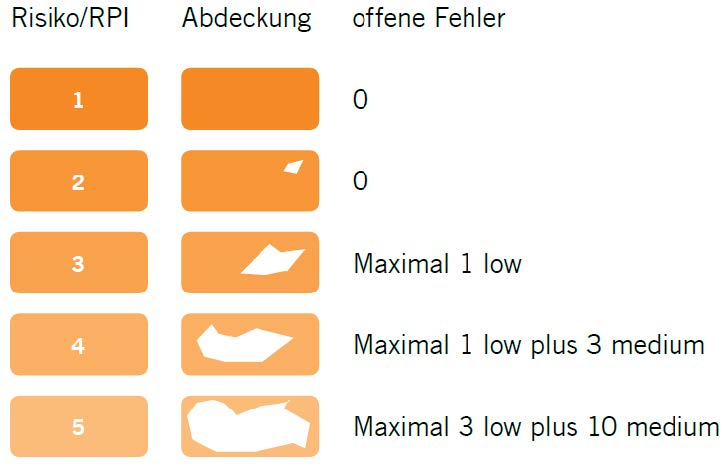
\includegraphics[width=0.6\linewidth]{fig/go-nogo-report}
\caption{Management Report}
\label{fig:go-nogo-report}
\end{figure}

Es bietet sich auch an ein Testcockpit für ein Projekt einzurichten. Dort sieht man jederzeit das erwartete Resultat eines Tests gemäss Anforderungen und kann dadurch schnell auf Fehler reagieren.

\textbf{Kennzahlen} sind nicht nur im Testen wichtig, weil man etwas was man nicht messen kann auch nicht kontrollieren kann. So muss z.B. ein Pilot jederzeit seine Flughöhe und Geschwindigkeit messen können, um sein Flugzeug im Griff zu haben. Das Erfassen von Kennzahlen kann auch mit Fiebermessen verglichen werden. Mit der Feststellung, dass das Kind Fieber hat, wird es nicht gesünder. Mit der Bestätigung, dass das Kind Fieber hat, auch nicht. Jedoch beugt ein regelmässigen Gesundheitscheck oft einer plötzlichen und schweren Krankheit vor. Die Kennzahlen müssen also im Testprozess definiert werden und dienen dort als Führungsinstrument der Projektleitung und des Testmanagements.

Während des Testprozesses gibt es verschiedene Kennzahlen, welche wichtige Fragen beantworten. Nachfolgend werden diese Fragen aufgelistet und beschrieben welche Kennzahlen diese beantworten.
\begin{description}
	\item[Was darf es kosten?] Mit Testen kann ein Projekt \textit{vergoldet} werden. Deshalb muss man Kosten und Nutzen von Tests sorgfältig abwägen. Man kann beispielsweise jeden Use Case mit einem RPI bewerten und je mehr Risiko ein Use Case hat desto mehr Tests werden dafür geschrieben.
	\item[Sind wir bereit?] Um diese Frage zu beantworten muss man den Testfortschritt dokumentieren. Der Testfortschritt beinhaltet wie viele Testfälle erstellt werden müssen, wie viele sind bereits erstellt und wie lange dauert die Vorbereitung noch. Man sollte auch darauf achten wie viele Use Cases bereits mit Tests abgedeckt sind. Das Management kann dann den Fortschritt über die Zeit beobachten und die Reihenfolge der Testerstellung dem Risiko eines Use Cases anpassen. Dann kann entschieden werden, ob man bereit zum Testen ist. Tester und Q-Menschen sind nie bereit, dass birgt das Risiko die Testvorbereitung und Testinfrastruktur zu vergolden.
	\item[Ist es reif?] Um zu entscheiden ob eine Komponente reif ist, muss man beobachten wie viele Tests zur Verfügung stehen und wie viele davon schon getestet werden konnten. Natürlich muss man auch beachten wie viele Tests erfolgreich sind und wie viele noch zu testen sind. Der Reifegrad einer Komponente kann aus der Summe aller Fehler, der Summe der offenen Fehler und der Anzahl der erfolgreich getesteten Use Cases bestimmt werden.
	\item[Wagen wir es?] Am Schluss kann das Management mit dem Testreport, welcher im vorherigen Abschnitt beschrieben wurde, entscheiden ob der Release gewagt wird.
\end{description}

\section{Nichtfunktionale Anforderungen und der Testquadrant}

\subsection{NFA}

\begin{figure}[h!]
\centering
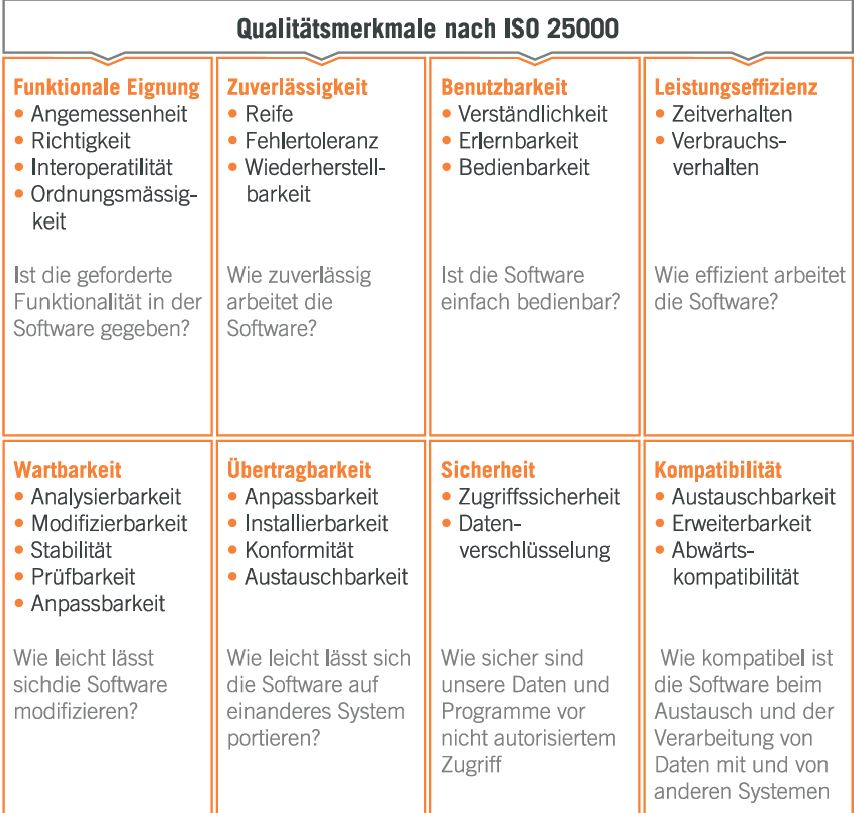
\includegraphics[width=0.56\linewidth]{fig/nfa-testing}
\caption{NFA Testing}
\label{fig:nfa-testing}
\end{figure}

\newpage

\subsection{Agile Testquadrant nach Brian Mark}

\begin{figure}[h!]
\centering
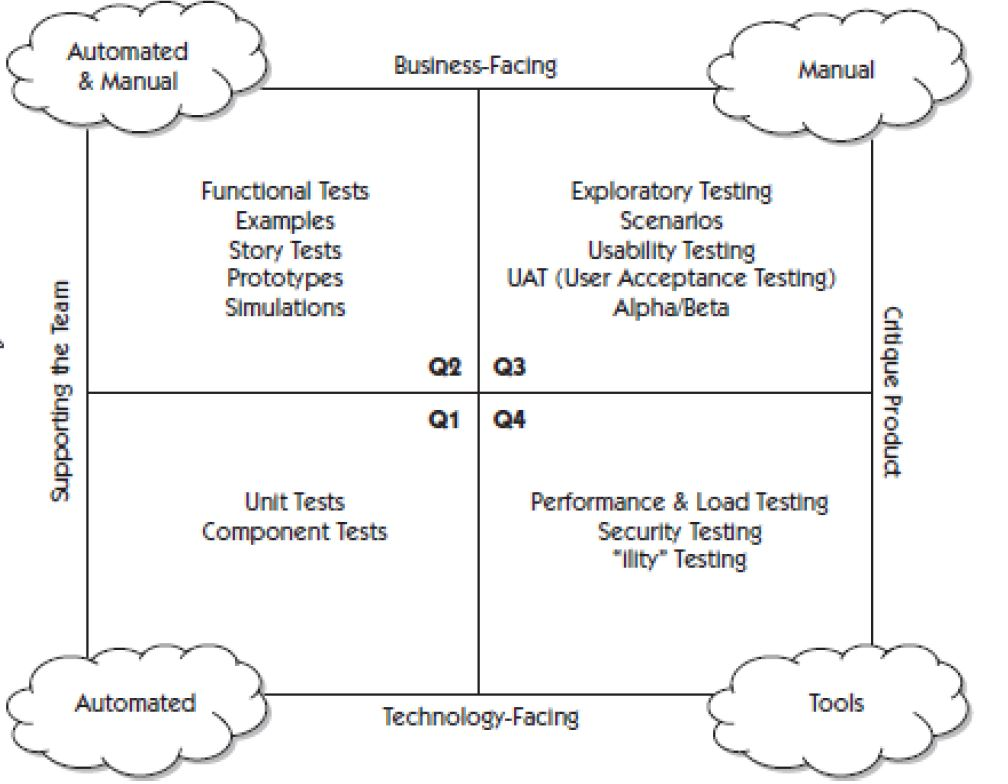
\includegraphics[width=0.5\linewidth]{fig/testquadrant}
\caption{Testquadrant}
\label{fig:testquadrant}
\end{figure}

\begin{description}
	\item[Quadrant 1 - unten links] Repräsentiert die Test getriebene Entwicklung - die Kernkomponente agiler Entwicklung. Die Unit- und Komponenten Tests in diesem Quadranten sind nicht unbedingt die ersten Tests die für eine bestimmte User Story geschrieben werden aber sie führen Design und Entwicklung an den richtigen Lösungsweg heran.
	
	\item[Quadrant 2 - oben links] Diese Tests unterstützt die Entwickler Teams auf einem höheren Niveau, denn sie sind am Geschäftsfall orientiert. Sie testen die extern wahrgenommene Qualität der vom Kunden definierten Features oder Anforderungen. Diese Tests treiben die Entwicklung auf einem höheren Level. Diese Tests werden von Business Experten leicht verstanden und aus diesem Grund in eine für sie lesbaren Sprache geschrieben. Hier auch - besser den Test vorher schreiben und erst danach implementieren. So kann der Entwickler es eigentlich gar nicht falsch implementieren. User Story sind oft zu unpräzise um den Need des Kunden genau zu spezifizieren. Daher eignet sich auch das Prototyping mit Hilfe diesen Tests.
	
	\item[Quadrant 3 - oben rechts] Das Reich der manuellen Tests! Es gibt exploratives, session-based, scenario sowie usability Testing. Darunter soll nicht nur die funktionalen Anforderungen getestet werden sondern auch die Nicht funktionalen Anforderungen. Beim explorativen Testen geht der Tester an die Software ran und schreibt quasi on the way die Testfälle und versucht "Fehler" zu finden. Diese haben sehr viel mit menschlicher Intelligenz sowie Intuition und Erfahrung zu tun. Daher sind diese schwer automatisierbar. Um hochwertige Software zu garantieren, reicht dieser Ansatz alleine nicht aus!
	
	\item[Quadrant 4 - unten rechts] Das Reich der NFA! In erster Linie werden hier nur NFA berücksichtigt. Dazu zählen wir Last-, Performance-, Security- und alle anderen ility-Tests. Obwohl sich diese Tests im letzten Quadranten befinden, sollen diese nicht erst am Schluss ausgeführt werden, sondern sobald wie möglich. Diese Tests können frühzeitig Schwachstellen der Architektur aufdecken. Probleme an dieser Stelle können zu grossen Umbauarbeiten führen. Die Erstellung dieser Tests ist mit grossem Aufwand verbunden. Für diese Tests sollten unbedingt entsprechende User Stories geschrieben werden - wobei Tool evaluiert werden und die Testumgebung definieren.
	
	\emph{Last- und Performance-Tests} erfordern oft erweitertes Fachwissen. Es braucht viel Vorlaufzeit und sind entsprechend aufwändig. Mittels Performance-Tests können Flaschenhälse im System ausgemacht werden. Load Tests stellen sicher, dass eine Applikation auch mit grosser Anzahl von gleichzeitigen Zugriffen fertig wird. Es gibt eine Reihe von Open Source Tools: JunitPerf, httperf, Apache JMeter, The Grinder, Pounder, ftptt, OpenWebLoad. Es gibt auch kommerzielle Tools. Die Evaluation und Einarbeitung in ein solches Tool braucht Zeit! Man sollte einmal eine Null-Linie definieren. Diese definiert den Ausgangspunkt von dem man sich verbessern möchte und kann so vergleichen - ob man wirklich Fortschritte erzielt. Es ist dabei wichtig, dass wir die Test reproduzierbar machen, in dem alle Faktoren dokumentiert werden (Hardware, System, Versionen usw.). Dabei sollte man sich auch immer um den Speicherverbrauch kümmern um allfälligen Memory-Leaks vorzubeugen - also messen! All diese Themen sollt ein Kapitel im Testplan gewidmet werden!
	
	Bei der \emph{Skalierbarkeit} geht es darum, dass auf einen Schlag mehr Benutzer die Applikation verwenden und das System diese doch verkraftet bzw. entsprechend skaliert werden kann.
	
	Für \emph{Security-Test} werden besser interne oder externe Spezialisten hinzugezogen. Sicherheitslöcher sind für eine Reputation einer Firma nicht gut und sollten dementsprechend prioritär behandelt weden.
	
	Die \emph{Wartbarkeit} kann nicht einfach so getestet werden. Sauber geschriebenen und kommentierten Code erhöhen die Wartbarkeit eines Systems. Es können Code-Guidlines definiert werden, allg. gültigste Standards und Konventionen sind einzuhalten, QS sollte auch Code- und Designreviews durchführen. Oder auch Pair-Programming oder die Clean-Code Bewegung sollten dazu führen.
	
	\emph{Kompatiblität und Interoperabilität} haben eine grosse Bedeutung wenn das System auf unterschiedlichen Systemen/Browser laufen muss. Das Testing kann schnell in ungeahnte Dimensionen steigen, wenn x-Geräte/Browser berücksichtigt werden müssen. Vielleicht sollte man auch auf Anbieter zurückgreifen, welche das für einen machen.
	
	\emph{Barrierefreiheit} - Kann die Applikation auch von sehbehinderten Menschen bedient werden? Warum grenzen wir diese aus?
	
	\emph{Zuverlässigkeit} beschäftigt sich mit der Frage, wie lange das System lauft bis es abstürzt oder einfriert. Kennzahlen sind hier MTF (mean time to failure) und MTBF (mean time between failures). Um das 1:1 testen zu können, braucht man oft einen langen Zeitraum um die Langzeitstabilität zu prüfen, was oft gar nicht möglich ist.
	
	Die \emph{Installierbarkeit} kann mit virtuellen Maschinen sehr gut und effizient verifiziert werden.
	 
\end{description}

\section{Praxisbeispiele}

Die Zufriedenheit eines End-Benutzer hängt massgebend davon ab, wie seine Erwartungen umgesetzt wurden. Diese Erwartungen sind als Anforderungen definiert und müssen verifiziert und validiert werden. Ein Test-Case beschreibt, wie eine Anforderung verifiziert wird. In einen Test-Case können mehrere Use-Cases und Anforderungen fliessen. Ein Use-Case beschreibt eine Sequenz von Aktionen, mit einem Resultat für den Aktor. Ein Use-Case sollte folgende Elemente beinhalten:
\begin{itemize}
	\item Name
	\item Kurze Beschreibung
	\item Ablauf
	\item Vorbedingungen
	\item Nachbedingungen
\end{itemize}
Abbildung \ref{fig:use-case-to-test-case} zeigt wie von einem Use-Case die entsprechenden Test-Cases abgeleitet werden.
\begin{figure}
\centering
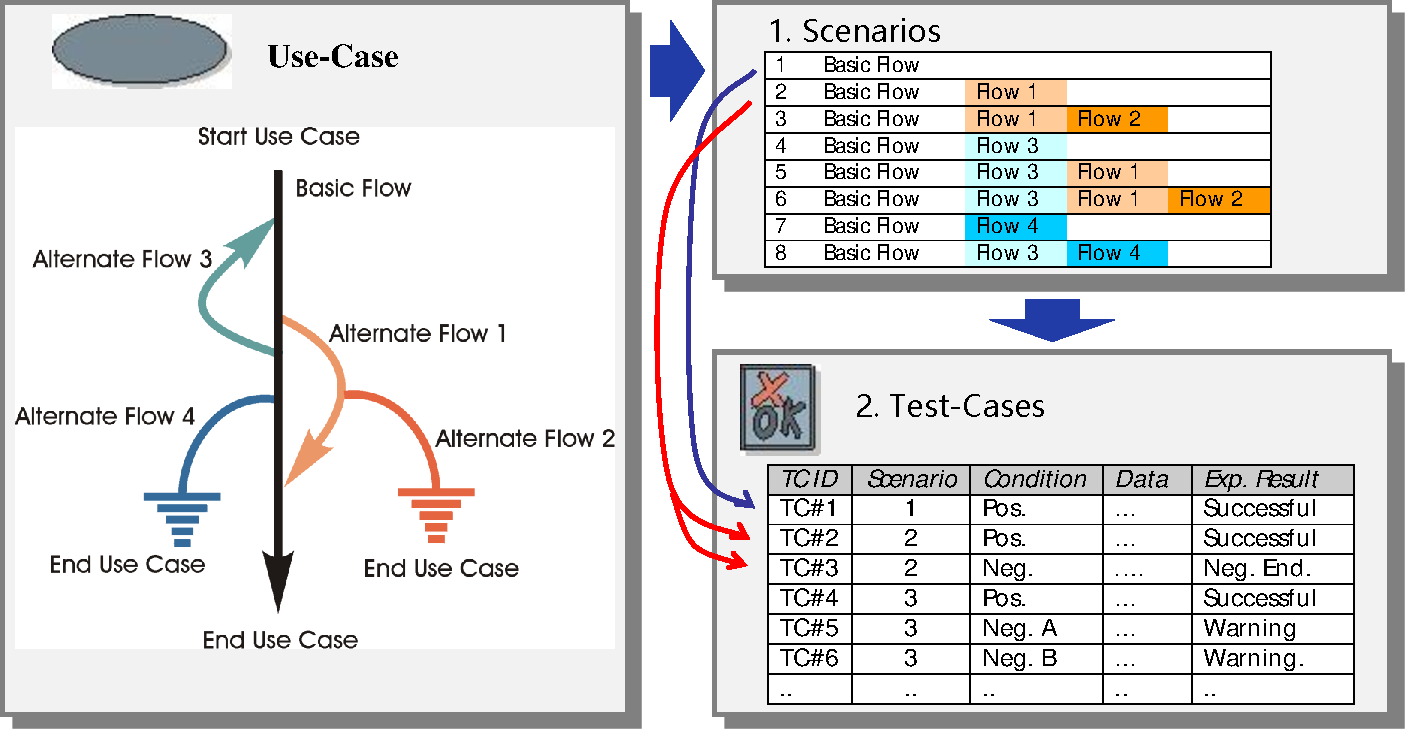
\includegraphics[width=0.7\linewidth]{fig/use-case-to-test-case}
\caption{Use Case in Test Case umwandeln}
\label{fig:use-case-to-test-case}
\end{figure}
Die Test-Cases können dann in einer Entscheidungstabelle gegenüber gestellt werden. Zudem kann der Test-Case um folgende Punkte ergänzt werden:
\begin{enumerate}
	\item Test-Case Description
	\item Execution Condition
		\begin{enumerate}
			\item Preconditions
			\item Test Inputs
			\item Observation Points
			\item Control Points
			\item Expected Results
			\item Postconditions
		\end{enumerate}
\end{enumerate}
Bei einem Test-Case ist weniger mehr, deshalb sollte der Test-Case agil wachsen. Als Best Practice sollte pro Anforderung mindestens zwei Test-Cases erstellt werden. Ein Test-Case zeigt, dass die Anforderung erfüllt ist und der zweite Test-Case prüft abnormales Verhalten. 

Nachfolgend wird ein Beispiel Schritt für Schritt aufgebaut, um das Erstellen eines Test-Cases zu erläutern. Wir nehmen an das du als Tester bei einer Versicherung arbeitest. Nun muss der Fall \textit{Mutterschaft} getestet werden. Es gelten folgende Regeln:
\begin{enumerate}
	\item Mutterschaft ist nur mit Geschlecht weiblich möglich
	\item Person muss versichert sein und gültige Versicherung haben
	\item Person muss in gültigem Altersbereich sein
	\item Der Zeitraum einer Schwangerschaft muss plausibel sein
\end{enumerate}
Als ersten Schritt müssen die Anforderungen geprüft und detailliert werden. So können beispielsweise folgende Fragen bezüglich der Anforderungen auftreten:
\begin{itemize}
	\item Was bedeutet z.B. gültige Versicherung?
	\item Was bedeutet gültiger Altersbereich?
	\item Was bedeutet plausibler Zeitraum?
\end{itemize}
Nachdem die Anforderungen widerspruchsfrei festgehalten wurden, beginnt die kreative Phase. Dabei überlegt man sich welche Testszenarien möglich sind. Man sollte besonders auf Spezialfälle und seltsame Situationen achten und diese als Szenarien festhalten. Sind die Testfälle grob umrissen können diese im Detail entwickelt werden.

Ein wichtiger Punkt sind auch die Testdaten. Grundsätzlich sollten pro Testszenario die jeweils notwendigen Testdaten spezifiziert werden. Dabei sollten folgende Punkte beachtet werden:
\begin{itemize}
	\item Wie kann sichergestellt werden, dass die Daten wiederverwendbar sind?
	\item Wie kann sichergestellt werden, dass die Daten auch nächstes Jahr noch gültig sind?
	\item Wo werden die Daten abgelegt?
	\item Wer verwaltet die Daten?
	\item Wer pflegt die Daten?
	\item Wer ist für die Daten verantwortlich?
\end{itemize}

\section{Testkonzept}

Idee:
\begin{itemize}
	\item Jeder Plan ist besser als kein Plan
	\item Schreiben ist exaktes Denken
	\item Testen bedingt einer Strategie
	\item Um WAS geht es > \emph{Big Picture}
	\item Ein- und Abgrenzen, um was geht es nicht
	\item Klären von Prioritäten (risikobasiert)
	\item Definieren des Vorgehens (Prozess) mit Hilfsmittel, Rollen und Verantwortlichkeiten
\end{itemize}

Struktur:
\begin{description}
	\item[Einleitung] Beinhaltet folgende Kapitel: Einleitung, Ziel u. Zweck, Geltungsbereich sowie geltende Dokumente u. Referenzen.
	
	\item[Testobjekt] Definition, welche Softwarekomponenten/Umsysteme getestet werden sollen (Scope) und was explizit nicht Bestandteil des Testprojekts ist (Constraints). Das Komponentendiagramm kann als Basis dienen, um die Testobjekte zu identifizieren.
	
	\item[Testumfang] Definition, welche Qualitätsmerkmale und Qualitätskriterien getestet werden sollen. Ein Qualitätsmerkmal hat als Ausprägung mehrere Qualitätskriterien. Qualitätsmerkmale: Funktionalität, Zuverlässigkeit, Effizienz, Benutzbarkeit. Qualitätskriterien: Richtigkeit, Angemessenheit, Stabilität, Performance.
	
	\item[Kommunikationswege] Beschreibt die Kommunikationswege der Mitglieder des Testprojekts je nach Rolle. Rollen: Projektleiter, Product Owner, Testmanager, Testengineer, Tester.
	
	\item[Risikobetrachtung] Einstufung der Risiken nach Eintrittswahrscheinlichkeit und Schweregrad. Falls diese schon im Rahmen eines Risikomanagements geführt werden, kann hier auf das entsprechende Dokument verweisen werden. Für jedes Risiko braucht es auch Massnahmen. Man unterscheidet zwischen Produkt- und Projektrisiko.
	
	\item[Lieferobjekte] Welche Lieferobjekte entstehen aus dem Testprojekt und wer ist Empfänger (Auftraggeber, Kunde)?  Hier sind Lieferobjekte zu nennen, welche sich nicht auf eine bestimmte Teststufe beziehen. Beispiele: Testkonzept, Dokumentation der Testumgebung, Testdaten, Status-Reports, Final-Reports, Testscripts, Automatisierungscode.
	
	\item[Teststufen u. Lieferobjekte] Definition, ob folgende Teststufen durchgeführt werden: Komponententests, Integrationstests, Systemtests, Abnahmetests.  Hier evtl. auch abhängige Lieferobjekte listen.
	
	\item[Komponententests/Unit-Tests] Werden Unit-Tests durchgeführt? Wer führt diese durch? Wo werden diese definiert/beschrieben? Der Entwickler macht in der Regel Unit-Tests direkt in der Entwicklungsumgebung. Es kann auch auf einzelne Teststufen verzichtet werden, bspw. macht man oft keine Unterscheidung zwischen System- und Integrationstests.
	
	\item[Planung] Falls die Projektplanung nicht genügend detailliert vorliegt, wird hier die Terminplanung mit Aktivitäten auf der Zeitachse ausgewiesen (GANT-Chart der einzelnen Iterationen).
	
	\item[Abnahmetests] Beschreibung ob und wie der Abnahmetest durchgeführt wird.
	
	\item[Testabbruch] Beschreibt Kriterien unter welche das Testing ganz oder teilweise abgebrochen wird resp. wieder aufgenommen wird. Projektleiter und Testmanager stehen in der Regel in der Verantwortung.
	
	\item[Testaktivitäten] Beschreibt, welche Aktivitäten vor, während und nach dem Testprojekt durchgeführt werden. Auch Aktivitäten, die explizit nicht durchgeführt werden, sollten vollständigkeitshalber beschrieben werden.
	
	\subitem Analyse / Vorbereitung: Studium der Testbasis, Entwurf der Testfälle, Aufbau der Testinfrastruktur.
	
	\subitem Durchführung / Auswertung: Funktionale Tests, Bugtracking, Zwischenbericht, nicht funktionale Tests in Bezug auf Effizienz, Stabilität, etc.
	
	\subitem Abschluss: Verfassen Abschlussbericht, Datenarchivierung, Abschlusspräsentation.
	
	\item[Personal] Beschreibt, wer welche Rolle innerhalb des Testprojekts hat, ob zusätzliches Personal rekrutiert werden muss oder ob Ausbildungsbedarf beim aktuell definierten Projektteam besteht.
	
\end{description}

Folgendes muss pro Teststufe dokumentiert werden:
\begin{description}
	\item[Testdesigntechniken] Beschreibung, wie die Testfälle hergeleitet werden. Beispiele: Review (Informell, Walktrough, Inspektion), Statische Analyse (Datenflussanalyse, Kontrollflussanalyse), Dynamische Analyse als Blackblox (Äquivalenzklassen, Grenzwertanalyse, Entscheidungstabelle Anwendungsfallbasiert).
	
	\item[Testendkriterien] Beschreibt, nach welchen Kriterien das Testende der jeweiligen Teststufe erreicht ist und die Tests als abgeschlossen betrachtet werden. Hierbei sollen qualitative Aspekte und nicht monetäre oder zeitliche Aspekte genannt werden. Beispiel: Alle Testfälle mit der Priorität Critical verlaufen erfolgreich und maximal 10\% der nicht kritischen Testfälle schlagen fehl.
	
	\item[Testmetriken] Beschreibt, welche Metriken während des Tests auf der jeweiligen Teststufe erhoben werden auf den Ebenen: Anforderungen, Testfälle, Testsets, Incidents/Defects. Dabei kann auf vorhandene Metriken des entsprechenden Testmanagementtools zurückgegriffen werden. Beispiel Anforderungen: Anzahl Anforderungen, bei denen die Testfälle erfolgreich durch geführt werden konnten, resp. ein oder mehrere Testfälle fehlschlugen. Beispiel Testfälle: Anzahl Testfälle mit den Status Passed und Failed.
	
	\item[Anforderungen an Testdaten] Spezifiziert, welche Testdaten erstellt werden und wo diese abgelegt/verwaltet sind. Beispiele: Stammdaten des Kunden, Daten von Vorgängerversionen, Von Testing erstellte Skripte.
	
	\item[Anforderungen an die Testumgebung] Beschreibt die Testumgebung (Software u. Hardware), sowie die abhängigen Umsysteme, die Einfluss auf die Testumgebung haben. Dabei soll auch die Version der entsprechenden Systeme angegeben werden. Beispiel: Der Versionsstand darf während einer Testiteration nicht verändert werden. Dies betrifft ebenfalls Änderungen, die die Konfiguration betreffen und nicht direkt im Programmcode definiert sind.
	
	\item[Regressionstests und Fehlernachtests] Beschreibt, wie Testfälle identifiziert werden, die in der nächsten Iteration wiederum getestet werden. Ferner wird definiert, wie mit Incidents/Defects umgegangen wird, resp. wie der Prozess hierfür definiert ist.
\end{description}

\begin{figure}[h!]
\centering
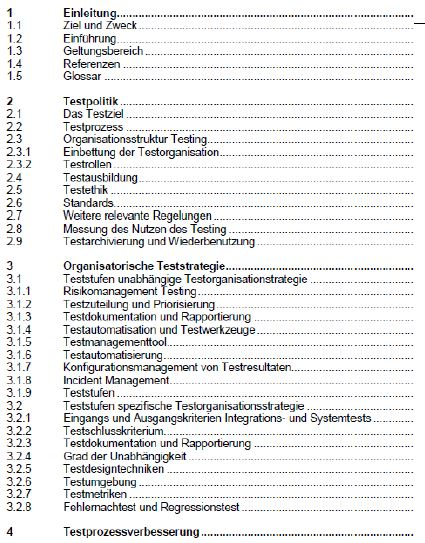
\includegraphics[width=0.6\linewidth]{fig/testkonzept-struktur}
\caption{Testkonzept-Struktur}
\label{fig:testkonzept-struktur}
\end{figure}
